\documentclass{beamer}
\usepackage{pgfplots}
\usepackage{tikz}
\pgfplotsset{compat=1.15}
\usepackage{mathrsfs}
\usetikzlibrary{arrows}
%\usepackage{pgfpages}
%\setbeameroption{show notes on second screen=right}
%setup images
\usepackage{graphicx}
\graphicspath{{./pics/}}
%equations and vectors
\usepackage[arrowdel]{physics}
\usepackage[normalem]{ulem}
\usepackage{amsmath,amssymb}
\usepackage{enumerate}
%theme
\usetheme[numbering=counter,progressbar=none,sectionpage=simple]{metropolis}
%references
%\usepackage[backend=biber,citestyle=authoryear,bibstyle=numeric,autocite=footnote,firstinits=true]{biblatex}
%\DeclareNameAlias{default}{family-given}
%\addbibresource{references.bib}
%\renewcommand*{\bibfont}{\scriptsize}
%\setbeamertemplate{bibliography item}[text]
%\renewcommand*{\nameyeardelim}{\addcomma\space}
%theme colors
\definecolor{mGreen}{HTML}{001514} %dark green for titles and frame headings
\definecolor{mBrown}{HTML}{422e24} %dark brown text
\definecolor{mEm}{HTML}{00625d} %light green for emphasis
\definecolor{mBg}{HTML}{ebe5d4} %background tan
\setbeamercolor{normal text}{fg=mBrown,bg=mBg}
\setbeamercolor{example text}{fg=mBrown,bg=mBg}
\setbeamercolor{title separator}{fg=mGreen}
\setbeamercolor{title}{fg=mGreen}
\setbeamercolor{subtitle}{fg=mBrown}
\setbeamercolor{frametitle}{bg=mGreen, fg=mBg}
%custom footnotes
\newcommand{\customfootnotetext}[2]{{
\renewcommand{\thefootnote}{#1}
\footnotetext[0]{#2}}}

\newcommand{\kk}{\frac{1}{4\pi\epsilon_0}}
\title{Electric Dipoles}
\subtitle{\small \emph{Analysing force and potential}}
\date{\today}
\author{Zella Baig}
%\institute{St. Hilda's College}
\begin{document}
\maketitle
\begin{frame}{Important Equations}
	\Large
		 \begin{equation}
			W= F \cdot s \cdot \cos \theta
		\end{equation}
		\begin{align}
			\va*  F &= \frac{1}{4\pi \epsilon_0} \frac{Q_{source}q_{test}}{r^2}  {\color{mEm}{\vu*r}} = \va*{E}q\\
			\va*{E} &= \frac{1}{4\pi\epsilon_0} \frac{Q}{r^2} \vu*{r} \: (V/m)\\
			V &= \frac{1}{4\pi\epsilon_0} \frac{Q}{r} \: (V) = \frac{W}{q}
		\end{align}
\end{frame}
\pgfplotsset{compat=newest}
\begin{frame}{The Task}
	\center{
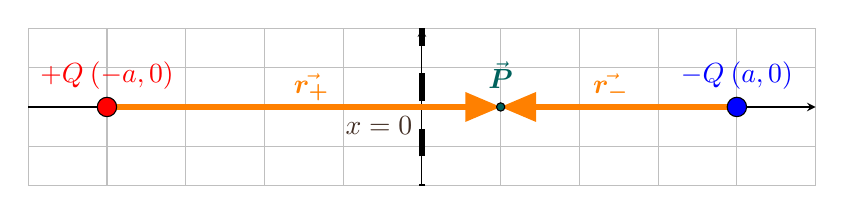
\begin{tikzpicture}[>=triangle 45,x=2cm,y=5cm]
\begin{axis}[
		x=2cm,y=5cm,
scale only axis,
ymajorgrids=true,
xmajorgrids=true,
xmin=-2.5,
axis lines=middle,
xmax=2.5,
ymin=-0.2,
ymax=0.2,
ticks=none,
]
\clip(-2.600001889534884,-0.8284883720930234) rectangle (2.600001889534884,0.5);
\draw [line width=2pt,dash pattern=on 10pt off 10pt] (0,-0.8284883720930234) -- (0,0.5);
\draw [->,line width=2pt,color=orange] (-2,0) -- (0.5,0);
\draw [->,line width=2pt,color=orange] (2,0) -- (0.5,0);
\draw[color=mBrown] (0,0) node[anchor=north east] {$x=0$};
\begin{scriptsize}
\draw [fill=blue] (2,0) circle (3.5pt);
\draw[color=blue] (2,0.08) node {$-Q \: (a,0)$};
\draw [fill=red] (-2,0) circle (3.5pt);
\draw[color=red] (-2,0.08) node {$+Q \: (-a,0)$};
\draw [fill=mEm] (0.5,0) circle (1.5pt);
\draw[color=mEm] (0.5,0.08) node {$ \va*{P}$};
\draw[color=orange] (1.2,0.05) node {$ \va*{r_{-}}$};
\draw[color=orange] (-0.7,0.05) node {$ \va*{r_{+}}$};
\end{scriptsize}
\end{axis}
\end{tikzpicture}}
	\Large
	What is the:
	\begin{enumerate}[a)]
	\item Force on a particle of charge $q$ located at point $ \va*{P}$ on the $x$ axis, as $ \va*{P}$ varies?
	\item Potential at point $ \va*{P}$ (if $V$ at $\infty = 0$) as $ \va*{P}$ varies?
	\end{enumerate}
\end{frame}
\begin{frame}{a) The Force at $ \va*{P}$}
\Large
	\begin{align*}
		\va*{E_{+}} = \frac{1}{4 \pi \epsilon_0} \frac{\left( +Q \right)}{r_{+}^{2}} \vu*{r_+}  
	\end{align*}
	\centering{but we are only considering the $x$ axis so:}
	\begin{align*}
		\va*{E_{+}} &= \frac{1}{4 \pi \epsilon_0} \frac{Q }{r_{+}^{2}} \vu*{x}  \\
		\rightarrow \va*{F_{+}} &= \frac{1}{4 \pi \epsilon_0} \frac{Q q}{r_{+}^{2}} \vu*{x}  
	\end{align*}
\end{frame}
\begin{frame}{a) The Force at $ \va*{P}$}
\Large
	\centering now for $ \va*{E_{-}}$:
	\begin{align*}
		\va*{E_{-}} &= \frac{1}{4 \pi \epsilon_0} \frac{\left( -Q \right)}{r_{-}^{2}} \vu*{r_-} \\
		&\rightarrow \text{where does $ \vu*{r_{-}}$ point?}
	\end{align*}
\end{frame}
\begin{frame}{a) The Force at $\va*{P}$}
\Large \centering
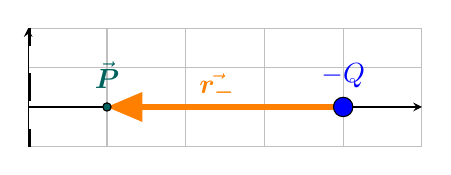
\begin{tikzpicture}[>=triangle 45,x=2cm,y=5cm]
\begin{axis}[
		x=2cm,y=5cm,
scale only axis,
ymajorgrids=true,
xmajorgrids=true,
xmin=0,
axis lines=middle,
xmax=2.5,
ymin=-0.1,
ymax=0.2,
ticks=none,
]
\clip(-2.600001889534884,-0.8284883720930234) rectangle (2.600001889534884,0.5);
\draw [line width=2pt,dash pattern=on 10pt off 10pt] (0,-0.8284883720930234) -- (0,0.5);
%\draw [->,line width=2pt,color=orange] (-2,0) -- (0.5,0);
\draw [->,line width=2pt,color=orange] (2,0) -- (0.5,0);
%\draw[color=mBrown] (0,0) node[anchor=north east] {$x=0$};
\begin{scriptsize}
\draw [fill=blue] (2,0) circle (3.5pt);
\draw[color=blue] (2,0.08) node {$-Q$};
%\draw [fill=red] (-2,0) circle (3.5pt);
%\draw[color=red] (-2,0.08) node {$+Q \: (-a,0)$};
\draw [fill=mEm] (0.5,0) circle (1.5pt);
\draw[color=mEm] (0.5,0.08) node {$ \va*{P}$};
\draw[color=orange] (1.2,0.05) node {$ \va*{r_{-}}$};
%\draw[color=orange] (-0.7,0.05) node {$ \va*{r_{+}}$};
%\draw[color=mBrown] (2.5,0) node[anchor= north east] {$x $};
\end{scriptsize}
\end{axis}
\end{tikzpicture}
	\begin{equation*}
		\rightarrow \vu*{r_{-}} = - \vu*{x}
	\end{equation*}
\end{frame}
\begin{frame}{a) The Force at $ \va*{P}$}
\Large
	\centering so:
	\begin{align*}
		\va*{E_{-}} &= \frac{1}{4 \pi \epsilon_0} \frac{\left( -Q \right)}{r_{-}^{2}} (-\vu*{x}) \\
		\va*{E_{-}} &= \frac{1}{4 \pi \epsilon_0} \frac{Q }{r_{-}^{2}} \vu*{x}\\
		\rightarrow \va*{F_{-}} &= \frac{1}{4 \pi \epsilon_0} \frac{Q q}{r_{-}^{2}} \vu*{x}  
	\end{align*}
\end{frame}
\begin{frame}{The Force at $\va*{P}$}
	\Large 
	\begin{align*}
		\va*{F_{total}} &= \va*{F_{+}} + \va*{F_{-}} \\
		&= \frac{Qq}{4\pi \epsilon_0} \left( \frac{1}{r_{+}^{2}} + \frac{1}{r_{-}^{2}}   \right)\vu*{x} \: (N)\\
		&\neq 0 \text{ at origin!}
	\end{align*}
\end{frame}
\begin{frame}{The Potential at $ \va*{P}$}
\Large
	\begin{align*}
		V_{+} &= \kk{} \frac{\left( +Q \right)}{r_{+}}  &V_{-} &= \kk \frac{\left( -Q \right)}{r_{-}}\\  
	\end{align*}
\end{frame}
\begin{frame}{The Potential at $ \va*{P}$}
	\Large
	\begin{align*}
		V_{total} &=  V_{+}+V_{-} = \frac{Q}{4\pi\epsilon_0}\left( \frac{1}{r_{+}}- \frac{1}{r_{-}}   \right) \: (V) \\
		&\rightarrow \text{\textbf{is }} 0 \text{ at origin!}
	\end{align*}
\end{frame}
\begin{frame}{Why Potential is $0$ at the Origin}
%\definecolor{ududff}{rgb}{0.30196078431372547,0.30196078431372547,1}
%\definecolor{uuuuuu}{rgb}{0.26666666666666666,0.26666666666666666,0.26666666666666666}
	\centering
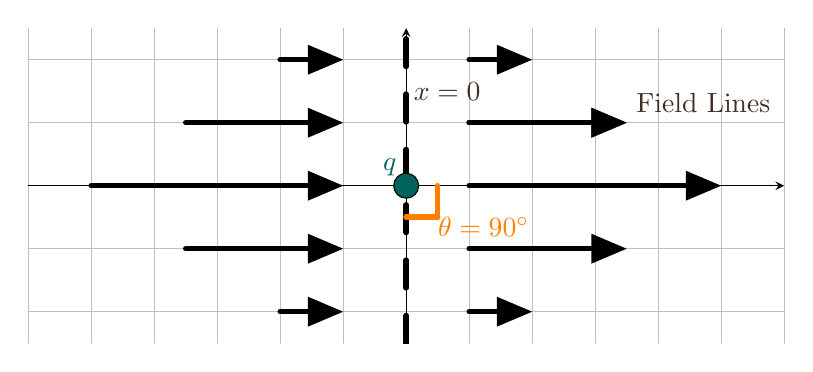
\begin{tikzpicture}[line cap=round,line join=round,>=triangle 45,x=1cm,y=1cm]
\begin{axis}[
x=4cm,y=4cm,
axis lines=middle,
ymajorgrids=true,
xmajorgrids=true,
xmin=-1.2,
xmax=1.2,
ymin=-0.5,
ymax=0.5,
ticks=none,]
\clip(-1.2,-1.8) rectangle (1.2,1.8);
\draw [line width=2pt,dash pattern=on 10pt off 10pt] (0,-0.5) -- (0,0.5);
\draw [->,line width=2pt] (0.2,0) -- (1,0);
\draw [->,line width=2pt] (0.2,0.2) -- (0.7,0.2);
\draw[color=mBrown] (0.7,0.2) node[anchor = south west] {Field Lines};
\draw [->,line width=2pt] (0.2,0.4) -- (0.4,0.4);
\draw [->,line width=2pt] (0.2,0.2) -- (0.7,0.2);
\draw [->,line width=2pt] (-1,0) -- (-0.2,0);
\draw [->,line width=2pt] (-0.7,0.2) -- (-0.2,0.2);
\draw [->,line width=2pt] (-0.4,0.4) -- (-0.2,0.4);
\draw [->,line width=2pt] (0.2,-0.2) -- (0.7,-0.2);
\draw [->,line width=2pt] (0.2,-0.4) -- (0.4,-0.4);
\draw [->,line width=2pt] (-0.4,-0.4) -- (-0.2,-0.4);
\draw [->,line width=2pt] (-0.7,-0.2) -- (-0.2,-0.2);
\draw [line width=2pt,color=orange] (0,-0.1)-- (0.1,-0.1);
\draw [line width=2pt,color=orange] (0.1,0)-- (0.1,-0.1);
\begin{scriptsize}
\draw[color=mBrown] (0.13,0.3) node {$x=0$};
\draw [fill=mEm] (0,0) circle (4.5pt);
\draw[color=mEm] (0,0) node[anchor = south east] {$q$};
\draw[color=orange] (0.07,-0.07) node[anchor = north west] {$\theta=90^{\circ}$};
\end{scriptsize}
\end{axis}
\end{tikzpicture}\\
\centering Recall that $W = F \cdot s \cdot \cos \theta$; but here $\cos \theta = \cos 90 = 0$, so:
\begin{align*}
	V = \frac{W}{q} = \frac{F \cdot s \cdot 0}{q} = 0 \text{ along $x=0$!}
\end{align*}
\end{frame}
\end{document}
